\documentclass[main.tex]{subfiles}
\begin{document}

\section*{Tue Oct 29 2019}

Recall the equations from last time: continuity, momentum and energy conservation in the isothermal case:
%
\begin{subequations}
\begin{align}
  \dot{M}  &= 4 \pi r^2 \rho v  \\
  v \dv{v}{r} &= - \frac{1}{\rho } \dv{P}{r} - \frac{GM}{r^2} \\
  T(r) &\equiv T 
\,.
\end{align}
\end{subequations}

Also, by differentiating the ideal gas law \(P \mu = \mathcal{R} T \rho \) we get
%
\begin{equation}
  \frac{1}{\rho } \dv{P}{r} = \frac{\mathcal{R} T}{\mu } \frac{1}{\rho } \dv{\rho }{r} 
  \marginnote{Divided through by \(\rho \).}
\,,
\end{equation}
%
since the temperature is constant.

Using this, we manipulate the momentum equation into 
%
\begin{align}
  v \dv{v}{r}  &= - \frac{1}{\rho } \frac{\mathcal{R} T}{\mu } \dv{\rho }{r} - \frac{GM}{r^2} 
\,,
\end{align}
%
but we know by the continuity equation that the density gradient must correspond to the velocity gradient:
%
\begin{equation}
  - \frac{1}{\rho } \dv{\rho }{r} = \frac{1}{v} \dv{v}{r} + \frac{2}{r}     
\,,
\end{equation}
%
which we can substitute into the equation: we get
%
\begin{align}
    v \dv{v}{r}  &=  \frac{\mathcal{R} T}{\mu } \qty(\frac{1}{v} \dv{v}{r} + \frac{2}{r}) - \frac{GM}{r^2} 
  \,.
\end{align}

It is a known fact that the isothermal speed of sound is given by 
%
\begin{equation}
  a^2 = \pdv{P}{\rho } =\pdv{}{\rho } \qty(\frac{\mathcal{R} \rho T}{\mu }) = \frac{\mathcal{R} T }{\mu }
  \implies
  a = \sqrt{\frac{\mathcal{R} T}{\mu }}
\,,
\end{equation}
%
so 
%
\begin{align}
    v \dv{v}{r}  &=  a^2 \qty(\frac{1}{v} \dv{v}{r} + \frac{2}{r}) - \frac{GM}{r^2} 
  \,.
\end{align}

Now we move all the terms which are proportional to the velocity gradient on the LHS: 
%
\begin{equation}
  \dv{v}{r} \qty(v - \frac{a^2}{v}) = \frac{2a^2 }{r }-\frac{GM}{r^2}
\,,
\end{equation}
%
which can be written as
%
\begin{equation}
    \frac{1}{v}\dv{v}{r} \qty(v^2 - a^2) = \frac{2a^2 }{r }-\frac{GM}{r^2}
  \,,
\end{equation}
%
so the Jacobian of the differential equation is zero is singular in \(v=a\): if \(v=a\) we must have \(2a^2r = GM\), which fixes the radius to the so-called Parker radius: \(r_P = GM / 2 a^2\), which is obtained by setting the LHS of the equation to zero.
Close to the star, the speed is subsonic (\(v < a\)), so the denominator \(D\) is negative; also the numerator \(N\) is negative in 
%
\begin{equation}
  \frac{1}{v} \dv{v}{r} 
  = \frac{2 a^2 / r - GM/ r^2}{v^2- a^2}
  \overset{\text{def}}{=} \frac{N}{D}
\,,
\end{equation}
%
so on the whole \(N/D\) is positive,
which is consistent with our assumption \(\dv*{v}{r} > 0 \), which we make since we are considering winds, as opposed to accretion. 

\begin{bluebox}
Why is the numerator negative? This is equivalent to saying 
%
\begin{align}
2 \frac{\mathcal{R} T}{\mu } < \frac{GM}{r}
\,,
\end{align}
%
which means that \(\Circled{B} \times 4/5 < \Circled{C}\), (using the notation from equation \eqref{eq:energy-conservation-differential}) which holds since, as we wrote there, \(\Circled{B} \ll \Circled{C} \) near the stellar radius. 
\end{bluebox}

Far from the star the numerator is positive, so the speed must be supersonic, so that \(N>0\) and we can still have \(N/D>0\) everywhere, guaranteeing that the velocity gradient is always positive.

So, the only physical solution is transsonic.

The critical velocity \emph{must} be attained at the Parker radius in order to have a physically meaningful transsonic solution; always-subsonic and always supersonic solutions are mathematically possible but not usually observed.

The velocity gradient at the critical point can be found by de l'Hôpital's rule to be 
%
\begin{equation}
  \dv{v}{r} \bigg|_{r_P} = \pm \frac{a^3}{GM}
\,.
\end{equation}

\begin{bluebox}
This is calculated by expanding in \(r\); however note that we must vary both \(r\) and \(v\) when we differentiate with respect to \(r\). We find: 
%
\begin{subequations}
\begin{align}
\dv{v}{r} &= v \frac{2 a^2 / r - GM/ r^2}{v^2- a^2}  \\
&= \bigg(a + \underbrace{\dv{v}{r}}_{\text{Second order}}\bigg)
\frac{- 2 a^2/r_P^2 + 2 GM / r_P^3}{2 a \dv*{v}{r}} \marginnote{Differentiated above and below at \(r = r_P\) and \(v =a \)}  \\
\qty(\dv{v}{r})^2 &=  - \frac{a^2}{r_P^2} + \frac{GM}{r_P^3} \marginnote{Simplified the \(2a\)}  \\
&= -a^2 \qty(\frac{2a^2}{GM})^2 + GM \qty(\frac{2a^2}{GM})^3  \marginnote{Substituted \(r_P = 2a^2 /GM\)}\\
&= -4 \frac{a^{6}}{(GM)^2} + 8 \frac{a^{6}}{(GM)^2}  \\
\dv{v}{r} & = \pm 2 \frac{a^3}{GM}
\,.
\end{align}
\end{subequations}
%
\end{bluebox}


\begin{claim}[Exercise]
The speed of sound at the critical point equals half of the escape velocity at that radius.
\end{claim}

\begin{bluebox}
The escape velocity is given by 
%
\begin{align}
v _{\text{esc}}^2 = \frac{2GM}{r}
\,,
\end{align}
%
but we know that \(r_P = GM / 2 a^2\): so 
%
\begin{align}
a^2 = \frac{GM}{2 r_P}
\,,
\end{align}
%
which means that, if we calculate the escape velocity at the Parker radius, we have \(v _{\text{esc}}^2 / a^2 = 4\), so \(v _{\text{esc}} / a = 2\). 
\end{bluebox}

There are exactly two transsonic solutions: if we trace a cross in the \(r, v\) plane centered on the critical point and speed of sound we see that all solutions meet it perpendicular to it. The solution with the decreasing velocity gradient is an accretion solution:
what is plotted is the \emph{absolute value} of the velocity, the accretion solution has always-negative absolute velocity gradient.

Always-supersonic solutions and always-subsonic ones are also found, but they do not obey the monotonicity of the velocity, so we discard them.

The boundary condition is the velocity at some \(r_0 \): the problem is second-order, but if we select the specific transsonic solution we eliminate the necessity of one boundary condition.
The choice we make for \(v_0  = v(r_0)\) is key, and nontrivial.

If we have the density, velocity and radius of the lower boundary we have \emph{fixed} the accretion rate: \(\dot{M}  = 4 \pi r_0^2 \rho_0 v_0 \). 

This is actually fixed by only specifying the gravity, temperature and density at the star's edge. It would seem like we also should have \(v_0 \), but we do not actually need it, as we will show in a moment.

With these hypotheses, we can solve the momentum equation analytically: we get 
%
\begin{subequations}
\begin{align} \label{eq:isothermal-wind-speed-equation}
\frac{v}{v_0 } \exp( -\frac{v^2}{2 a^2}) &= \qty(\frac{r_0}{r})^2 \exp(\frac{GM}{a^2} \qty(\frac{1}{r_0 } - \frac{1}{r}))  \\
&= \qty(\frac{r_0}{r})^2 \exp(\frac{2r_c}{r_0 } - \frac{2r_c}{r})
\,.
\end{align}
\end{subequations}
%

\begin{bluebox}
So, to calculate the Mach number we need to solve 
%
\begin{align} 
M e^{-M^2/2} = \frac{v_0 }{a} \qty(\frac{r_0 }{r})^2 \exp(\frac{2r_c}{r_0 } - \frac{2 r_c}{r})
\,,
\end{align}
%
but there seems to be an issue: the left hand side is bounded (it attains its maximum value of \(e^{-1/2} \approx 0.6\) at \(M=1\)) while the RHS is maximized at \(r = r_c\), where it is equal to 
%
\begin{align}
\frac{v_0}{a} \qty(\frac{r_0 }{r_c})^2 \exp(\frac{2r_c}{r_0 } - 2)
\,,
\end{align}
%
which is dependent on \(v_0 \)! If we plug in solar values for the parameters, \(T = \SI{1e6}{K}\), \(\mu = \num{.62}\) and select an initial velocity like \(v_0 = \SI{1}{km/s}\) we get that the RHS's maximum is around 35! 

This means that, in order to always have solutions, we need to fix \(v_0 \) to set the maxima to be equal.
This gives us 
%
\begin{subequations}
\begin{align}
v_0 &= e^{-1/2}  \qty(\frac{1}{a} \qty(\frac{r_0}{r_c})^2
\exp(\frac{2 r_c}{r_0 }) e^{-2})^{-1} \\
&= a \qty(\frac{r_c}{r_0 })^2 \exp(-  \frac{2r_c}{r_0 } + \frac{3}{2})
\,.
\end{align}
\end{subequations}

Specifically, we can see that for the solar values mentioned before \SI{1}{km/s} was an overestimate, and with the values we fixed the initial velocity is actually more like \SI{17}{m/s}.
\end{bluebox}

At large distances, we get \(v \rightarrow 2 a \sqrt{\ln(r/r_0)}\).

\begin{bluebox}
To derive this, take the log of the equation and take the limit \(r \rightarrow \infty \).
%
\begin{align}
-\frac{M^2}{2} + \log M 
= \log \frac{v_0 }{a} + 2 \log \frac{r_0 }{r} + \frac{2 r_c}{r_0 } - \frac{2 r_c}{r}
\,,
\end{align}
%
so the RHS diverges as \(- \log r\) does for \(r \rightarrow \infty\), which means that the LHS must also diverge and become very large and negative. The polynomial term \(-M^2/2\) dominates the logarithmic one.
So, asymptotically we have \(- M^2/2 \approx 2 \log r_0 /r \), which means \(M \approx 2 \sqrt{\log (r/r_0) }\).
\end{bluebox}
\todo[inline]{This is reported incorrectly in the slides as \(v \rightarrow 2 a \log (r / r_0 )\). }

This is unphysical (the velocity diverges!?) and due  to the fact that we assume a constant temperature (and, thus, energy input) even for diverging \(r\). 

The density profile can be found from the continuity equation to be 
%
\begin{align} \label{eq:isothermal-wind-density}
\frac{\rho}{\rho_0} \exp(\frac{1}{2} \qty(\frac{v_0 \rho_0 r_0^2}{a \rho r^2})^2) = \exp(2 r_c \qty(\frac{1}{r} - \frac{1}{r_0}))
\,,
\end{align}
%
\begin{figure}[H]
\centering
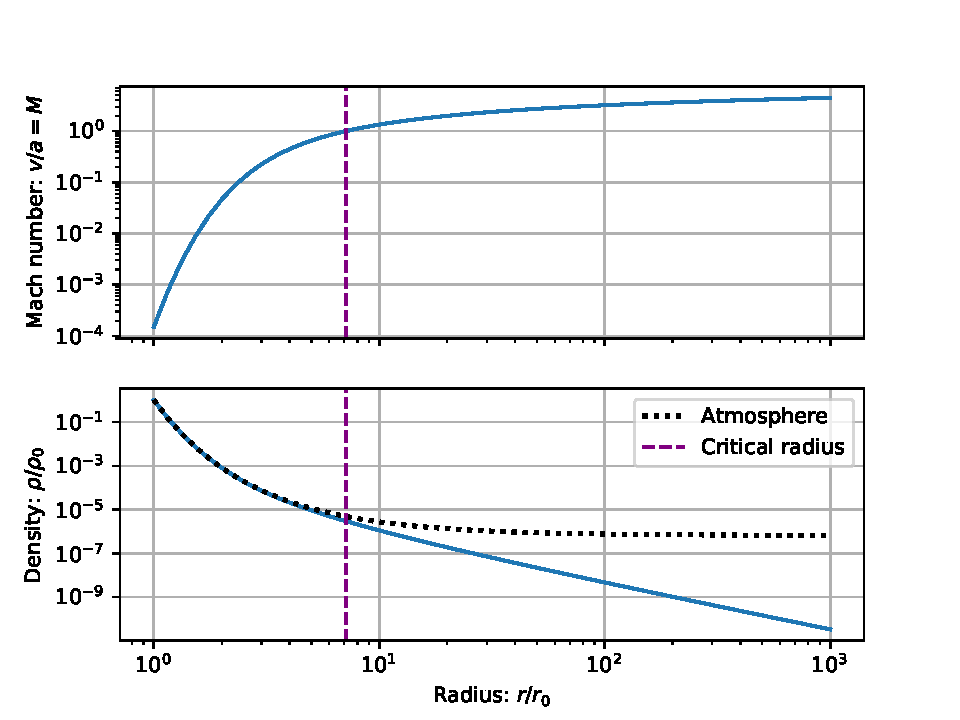
\includegraphics[width=\textwidth]{figures/atmosphere_critical_radius.pdf}
\caption{Velocity profile (solution to \eqref{eq:isothermal-wind-speed-equation}) and density wind profile (solution to \eqref{eq:isothermal-wind-density}), plus atmosphere (hydrostatic) profile (shown in \eqref{eq:density-profile-hydrostatic-equilibrium}).}
\label{fig:atmosphere_critical_radius}
\end{figure}
  

Now we look at the structure of the wind in the subcritical region.

In the corresponding slide: the dashed line in the density profile is the density we'd expect in a hydrostatic atmosphere, while the solid one is the solution.

The hydrostatic density structure is given by 
%
\begin{subequations}
\begin{align}
  \frac{1}{\rho } \dv{P}{r}  +\frac{GM }{r^2}  &= 0 
\,,
\end{align}
\end{subequations}
%
since we set the (log) velocity gradient to zero.
Manipulating this we get 
%
\begin{equation}
  \frac{r^2}{\rho } \dv{\rho }{r} = - \frac{GM}{a^2}
\,,
\end{equation}
%
So, integrating this we see that the density profile follows a decreasing exponential law: 
%
\begin{equation} \label{eq:density-profile-hydrostatic-equilibrium}
  \frac{\rho (r)}{\rho_0 } = \exp(\frac{-(r-r_0 )}{H_0 } \frac{r_0}{r} ) 
\,,
\end{equation}
%
where \(H_0 \) is the scale height, \(H_0 = \mathcal{R} T / \qty(\mu g_0 )\) with \(g_0 = GM / r_0^2\).
The length scale at which this decreases is defined by \(H_0 \). 

The density profile in the subsonic region is very well approximated by this hydrostatic profile: as we can see in figure \ref{fig:atmosphere_critical_radius} in the subsonic region the log-velocity gradient is small, so the pressure contribution dominates.

The mass loss rate is our main prediction: we have \(\dot{M } = 4 \pi r^2_0 \rho_0 v_0 = 4 \pi r_c^2\rho_c a\).

In order to compute it at the critical radius, we can use the density profile equation: 
%
\begin{equation}
  \dot{M} = 4 \pi r_c^2 a \rho_0 \exp(\frac{-(r_c - r_0 )}{H_0 } \frac{r_0 }{r_c}) 
\,.
\end{equation}
%
\todo[inline]{This is an approximation, justified by the fact that in the subsonic region the density profile of the wind is almost the same as in hydrostatic equilibrium. There is a correction factor of \(\exp(-1/2)\).}

If we consider this numerically, we find that the exponential is the dominant part: the mass loss rate becomes lower when the critical point moves outward.
We can specify it by fixing 
%
\begin{enumerate}
    \item the temperature at the corona, \(T_C\);
    \item the radius at the bottom of the corona, \(r_0 \);
    \item the stellar mass \(M\);
    \item the density at the bottom of the corona \(\rho_0 \).
\end{enumerate}

In the slides there are numerical estimates. 
As \(H_0 \) increases, the density profile is less steep: the density remains high at larger radii.

\begin{bluebox}
Why is the dependence on \((r_c - r_0 ) /H_0 \) so strong? The idea seems to be that in order for the wind to expel a significative quantity of material it needs to give it a large velocity in a small space, otherwise the wind becomes supersonic when its density is very small.
\end{bluebox}

\end{document}
